\documentclass{article}


\usepackage{PRIMEarxiv}

\usepackage[utf8]{inputenc} % allow utf-8 input
\usepackage[T1]{fontenc}    % use 8-bit T1 fonts
\usepackage{hyperref}       % hyperlinks
\usepackage{url}            % simple URL typesetting
\usepackage{booktabs}       % professional-quality tables
\usepackage{amsfonts}       % blackboard math symbols
\usepackage{nicefrac}       % compact symbols for 1/2, etc.
\usepackage{microtype}      % microtypography
\usepackage{siunitx}
\usepackage{hyperref}
\sisetup{per-mode=symbol}
\usepackage{lipsum}
\usepackage{parskip}
\usepackage{fancyhdr}       % header
\usepackage{graphicx}       % graphics
\graphicspath{{images/}}     % organize your images and other figures under media/ folder

%Header
\pagestyle{fancy}
\thispagestyle{empty}
\rhead{ \textit{ }} 

% Update your Headers here
\fancyhead[LO]{To the Moon By Water Balloon}
% \fancyhead[RE]{Firstauthor and Secondauthor} % Firstauthor et al. if more than 2 - must use \documentclass[twoside]{article}



  
%% Title
\title{To the Moon By Water Balloon}

\author{
  Seth Katz \\
  \texttt{\{katzseth22202@gmail.com} \\
}


\begin{document}
\maketitle


\begin{abstract}
    Project Orion \cite{projorion} proposed using nuclear explosions to accelerate a spacecraft.  Although Project Orion was cancelled for practical reasons,  it successfully demonstrated the theoretical feasibility of propelling spacecraft using pulses of gas impacting a shock-absorbing pusher plate.

    Instead of bombs, we can give the spacecraft momentum pulses by crashing low density balloons into a pusher plate at the back of the rocket fuselage.  We will call this idea balloon pulse propulsion \cite{aim2024}.
 \begin{figure}[h]
    \centering
    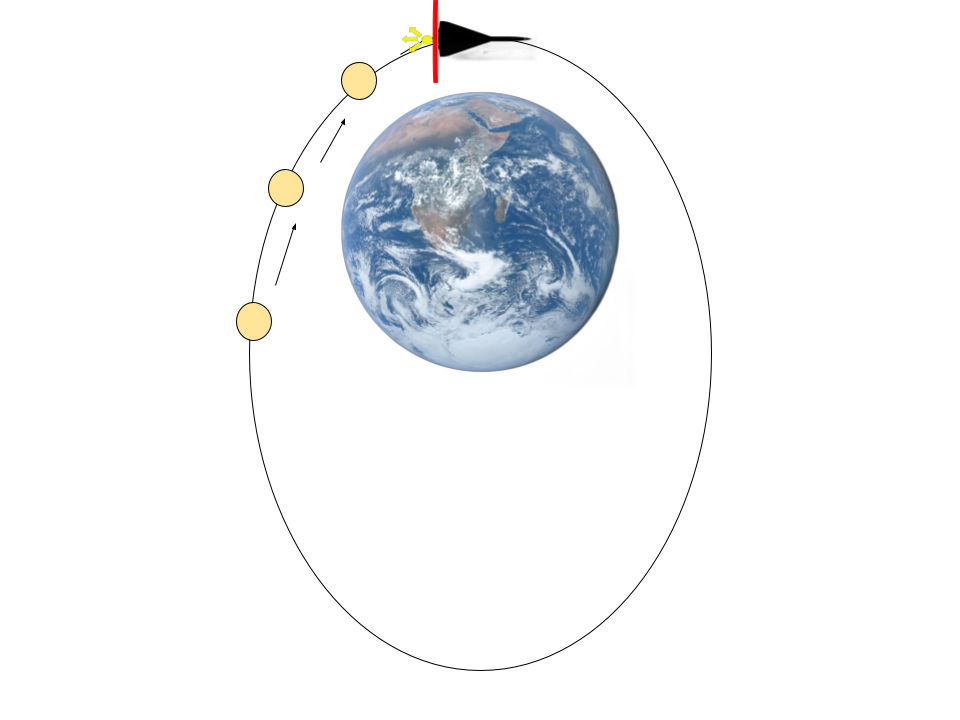
\includegraphics[width=0.5\linewidth]{images/Starship_Impact_ellipse.png}
    \caption{Starship can launch balloons in an ellipse.   A separate suborbital craft steers into the balloon path for momenum}
    \label{fig:starship_ellipse}
\end{figure}

As shown in \autoref{fig:starship_ellipse}, the balloons are launched into an eccentric orbit from a larger spacecraft, such as SpaceX Starship \cite{starship}.   Subsequently, a suborbital rocket launches from Earth and intercepts the path of the balloons just above the atmosphere.    

The suborbital rocket can take off with air breathing jet engines just like an airplane, igniting its rocket engines at high altitudes. Unlike SpaceX’s proposed Earth-to-Earth direct rocket travel \cite{spacex_earth_earth}, this suborbital rocket integrates seamlessly with today’s commercial aviation infrastructure. If desired, the rocket can be propelled into low Earth orbit instead of traveling to another city.

If the volatiles used to fill the balloons are sourced from lunar shadowed regions, asteroids, or distant low-gravity icy bodies, we can eliminate the need for heavy rockets to launch the balloons from Earth. Utilizing gravity assists and other techniques, these balloons can intercept Earth at extremely high speeds. Their kinetic energy can be harnessed to produce energy on an enormous scale.   This energy can be used in space but it can also be transferred to power human civilization on Earth.

The remainder of this proposal delves into the details of balloon pulse propulsion engineering and economic advantages. We then explore how materials sourced from the Moon or Ceres can eliminate the need for a Starship balloon rocket launch. Following this, we describe methods to generate clean terrestrial electricity from balloon kinetic energy. 

Achieving balloon pulse propulsion requires positioning the balloons with centimer  precision.  Proving this is feasible is a likely first step in validating the concept.    To attract private funding for a demonstration of this precision object deployment, we propose launching a rocket filled with thousands of kilogram-sized “meteors” to create spectacular artificial meteor showers on Earth above a few major cities. These showers could coincide with a special celebration, such as July 4th, and be visible to most Americans. We also outline the requirements and proposed budgets for this initial step.   Note private investor risk in mitigated because the meteor shower will likely be spectacular and enjoyable even if fail to achieve the desired precision of each object.   

\end{abstract}


\section{Balloon Pulse Propulsion Modelling}
\label{sec:pulse_modelling}
\subsection{Starship Economics - leveraging spare payload capacity for safer satellite launches}
SpaceX’s Starship has the potential to dramatically reduce launch costs if it achieves full reusability. However, its payload capacity is much larger than necessary for today’s satellite market, leading to capacity underutilization during satellite launches.   \begin{quote}
Carissa Christensen, the chief executive of Bryce Tech, an analytics firm that tracks the launch market, says launching Starship frequently will be key to closing SpaceX’s business case, but finding customers to fill the rocket’s giant payload capacity will be challenging. 
"Starship's payload capacity is huge; it's very, very big, and there aren't that many commercial uses today for a rocket that big," she said.  "Maybe it'll be so cheap that it makes sense to launch satellites on it if its not full or near full." \cite{nyt_starship_size}

In other words Starship satellite launches will underutilize payload capacity.   The launch cost may also fall significantly below the cost of building the satellite once launches are reusable and cheap.   With balloon pulse propulsion, we launch Starship at full payload with balloons.   Since the satellite is on a secondary rocket, it is never placed next to the fragile high propellant mass fraction orbital rocket.   We buy a safer launch with Starship's spare capacity when we employ balloon pulse propulsion and a secondary suborbital rocket.

\subsubsection{Balloon To Rocket Mass Launch Ratios}\label{sec:balloon_rocket_ratio}
Let's built a simplified model of how large a spacecraft a given mass of balloons can accelerate.

Suppose \(v_r\)\,  \(v_b\),  \(m_r\), and \(m_b\) represent balloon and rocket masses and velocities,    \(a\) represents the constant desired rocket acceleration and \(e\) represents how efficient each balloon collision is, where \(e=1\) would be a perfectly elastic collision.   For simplicity, let's assume the efficiency is the same for each balloon and that 1 balloon impacts the pusher plate each second.   Using the equations for elastic collisions shows that 
\begin{equation}
m_b=\frac{-am_r}{e(a - 2v_b + 2v_r)}
\label{eq:balloon_mass}
\end{equation}
We can write a simple script to loop and add the balloon masses until desired velocity is achieved.   If the final suborbital rocket speed is \SI{7.8}{\kilo\metre\per\second}, \(v_b=\SI{11}{\kilo\metre\per\second}\), and \(e=.6\) then the balloons can lift 112 \% of their mass into low Earth orbit.   

The collision efficiency can likely be improved by absorbing more of the light produces when the balloon gas heats up.   Project Orion assumed these collisions are highly efficient because the plasma was opaque to the radiation it produced \cite{orion_reflections}.  Our gas won't be hot enough to benefit from these calculations, but we can design the pusher plate to spray soot.   Since our pulses can be small, they can also potentially be partially contained by a pusher plate designed to reflect light many times though the gas to increase absorption.   The more of this radiation we absorb, the more efficient our pulses can be.  

Individual balloons traveling in elliptical orbits follow paths around the Earth’s center of mass. For intercity travel, adjustments are necessary since most cities are not connected by paths that bisect the Earth’s center. A suborbital rocket can make minor trajectory adjustments if the required correction is small. Alternatively, two balloon pulses can be used (see \autoref{fig:two_pulses}), where the second pulse adjusts the spacecraft’s trajectory to reach the destination city.

\begin{figure}
    \centering
    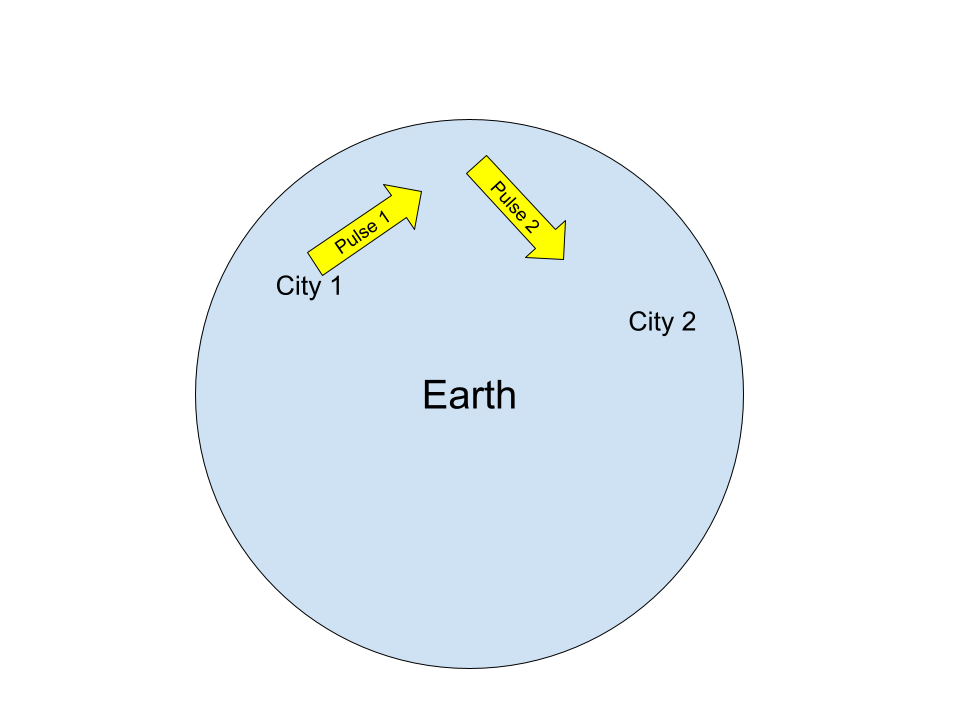
\includegraphics[width=0.5\linewidth]{images/Two Pulses.png}
    \caption{A first sequence of balloon pulses launches the spacecraft into orbit, then a second smaller set of pulses adjusts the orbit to target the second city}
    \label{fig:two_pulses}
\end{figure}
\subsection{Private Jet Travel and Oxygen Refuelling}
Currently, passenger aviation volume represents orders of magnitude more tonnage than satellites.  
\end{quote}  Airlines served nearly 4.5 billion yearly passengers before the COVID pandemic.  \cite{icao_passenger_volume}.  By contrast, only about 50,000 tons worth of satellites have ever been launched. \cite{usa_today_satellite}.    Starship's payload of 150 \SI{tonne}



\section{Balloon Pulse Propulsion Modelling}
\label{sec:pulse_modelling}
\subsection{Starship Economics and Balloon Pulse Propulsion}
SpaceX Starship will be reusable, but it also has an unnecessarily large payload capacity for almost any current satellites.   For example, 




\subsection{Suborbital rockets from ordinary airports}\label{sec:suborbital_airports}
SpaceX has proposed direct Earth to Earth transportation with SpaceX Starship \cite{spacex_earth_earth}.   However, in the unlikely event this received regulatory approval, it would require very complex bordering procedures involving boats to offshore platforms.   If we could use regular airports, the concept would be much more viable.    However, most airports don't have the liquid oxygen handling facilities for a rocket engine.

Since our suborbital plane has a low propellant mass fraction, we can spend some weight including air breathing jet engines for takeoff and landing.   The plane takes off with empty oxygen tanks.   Separately, a specialized oxygen airplane tanker takes off from specialized airports that do have liquid oxygen facilities.    The planes rendezvous and the tanker fuels the suborbital rocket's oxygen tank mid-air.   This is similar to military airplane refueling, except we are tanking up on oxygen rather than fuel.   The specialized oxygen handling airports can be in rural areas near major regions.   A tanker taking off in West Virginia could likely rendezvous with an airplane from any airport between Boston and Washington DC within half an hour of takeoff.   

Suborbital planes with heat shielding can reenter the atmosphere for landing.   However, heat shielding adds weight.   Sonic booms from reentry could create regulatory hurdles.   Alternatively, we can use balloon pulse propulsion to decelerate before atmospheric reentry.   Balloons into the retrograde orbit of the suborbital rocket.   Since these retrograde balloons don't need to be launched into a high elliptical orbit, significantly less mass would be required.

\section{Private Aviation Most Likely Initial Market}
SpaceX Starship payload to elliptical orbits like GTO is about 27 tons \cite{spacex_user_guide}.   This implies lifting approximately a 32 ton plane based on our balloon mass analysis in \autoref{sec:pulse_modelling}.   That is fairly small for a commercial airplane, but is comparable to a mid sized private jet.   Also, the Concorde's economic failure suggests passengers are unwilling to pay very high premiums for faster travel \cite{concorde_expensive}.  The wealthiest private jet customers presumably are less price sensitive and care more about saving time.



\subsection{Headings: second level}
\lipsum[5]
\begin{equation}
\xi _{ij}(t)=P(x_{t}=i,x_{t+1}=j|y,v,w;\theta)= {\frac {\alpha _{i}(t)a^{w_t}_{ij}\beta _{j}(t+1)b^{v_{t+1}}_{j}(y_{t+1})}{\sum _{i=1}^{N} \sum _{j=1}^{N} \alpha _{i}(t)a^{w_t}_{ij}\beta _{j}(t+1)b^{v_{t+1}}_{j}(y_{t+1})}}
\end{equation}

\subsubsection{Headings: third level}
\lipsum[6]

\paragraph{Paragraph}
\lipsum[7]

\section{Examples of citations, figures, tables, references}
\label{sec:others}
\lipsum[8] \cite{kour2014real,kour2014fast} and see \cite{hadash2018estimate}.

The documentation for \verb+natbib+ may be found at
\begin{center}
  \url{http://mirrors.ctan.org/macros/latex/contrib/natbib/natnotes.pdf}
\end{center}
Of note is the command \verb+\citet+, which produces citations
appropriate for use in inline text.  For example,
\begin{verbatim}
   \citet{hasselmo} investigated\dots
\end{verbatim}
produces
\begin{quote}
  Hasselmo, et al.\ (1995) investigated\dots
\end{quote}

\begin{center}
  \url{https://www.ctan.org/pkg/booktabs}
\end{center}


\subsection{Figures}
\lipsum[10] 
See Figure \ref{fig:fig1}. Here is how you add footnotes. \footnote{Sample of the first footnote.}
\lipsum[11] 

\begin{figure}
  \centering
  \fbox{\rule[-.5cm]{4cm}{4cm} \rule[-.5cm]{4cm}{0cm}}
  \caption{Sample figure caption.}
  \label{fig:fig1}
\end{figure}

\subsection{Tables}
\lipsum[12]
See awesome Table~\ref{tab:table}.

\begin{table}
 \caption{Sample table title}
  \centering
  \begin{tabular}{lll}
    \toprule
    \multicolumn{2}{c}{Part}                   \\
    \cmidrule(r){1-2}
    Name     & Description     & Size ($\mu$m) \\
    \midrule
    Dendrite & Input terminal  & $\sim$100     \\
    Axon     & Output terminal & $\sim$10      \\
    Soma     & Cell body       & up to $10^6$  \\
    \bottomrule
  \end{tabular}
  \label{tab:table}
\end{table}

\subsection{Lists}
\begin{itemize}
\item Lorem ipsum dolor sit amet
\item consectetur adipiscing elit. 
\item Aliquam dignissim blandit est, in dictum tortor gravida eget. In ac rutrum magna.
\end{itemize}


\section{Conclusion}
Your conclusion here

\section*{Acknowledgments}
This was was supported in part by......

%Bibliography
\bibliographystyle{unsrt}  
\bibliography{references}  


\end{document}
